\begin{figure}[htbp]
\centering
\caption{Predictors of Bilateral Connectivity}
\label{fig:bilateral_coefplot_combined}

\begin{threeparttable}

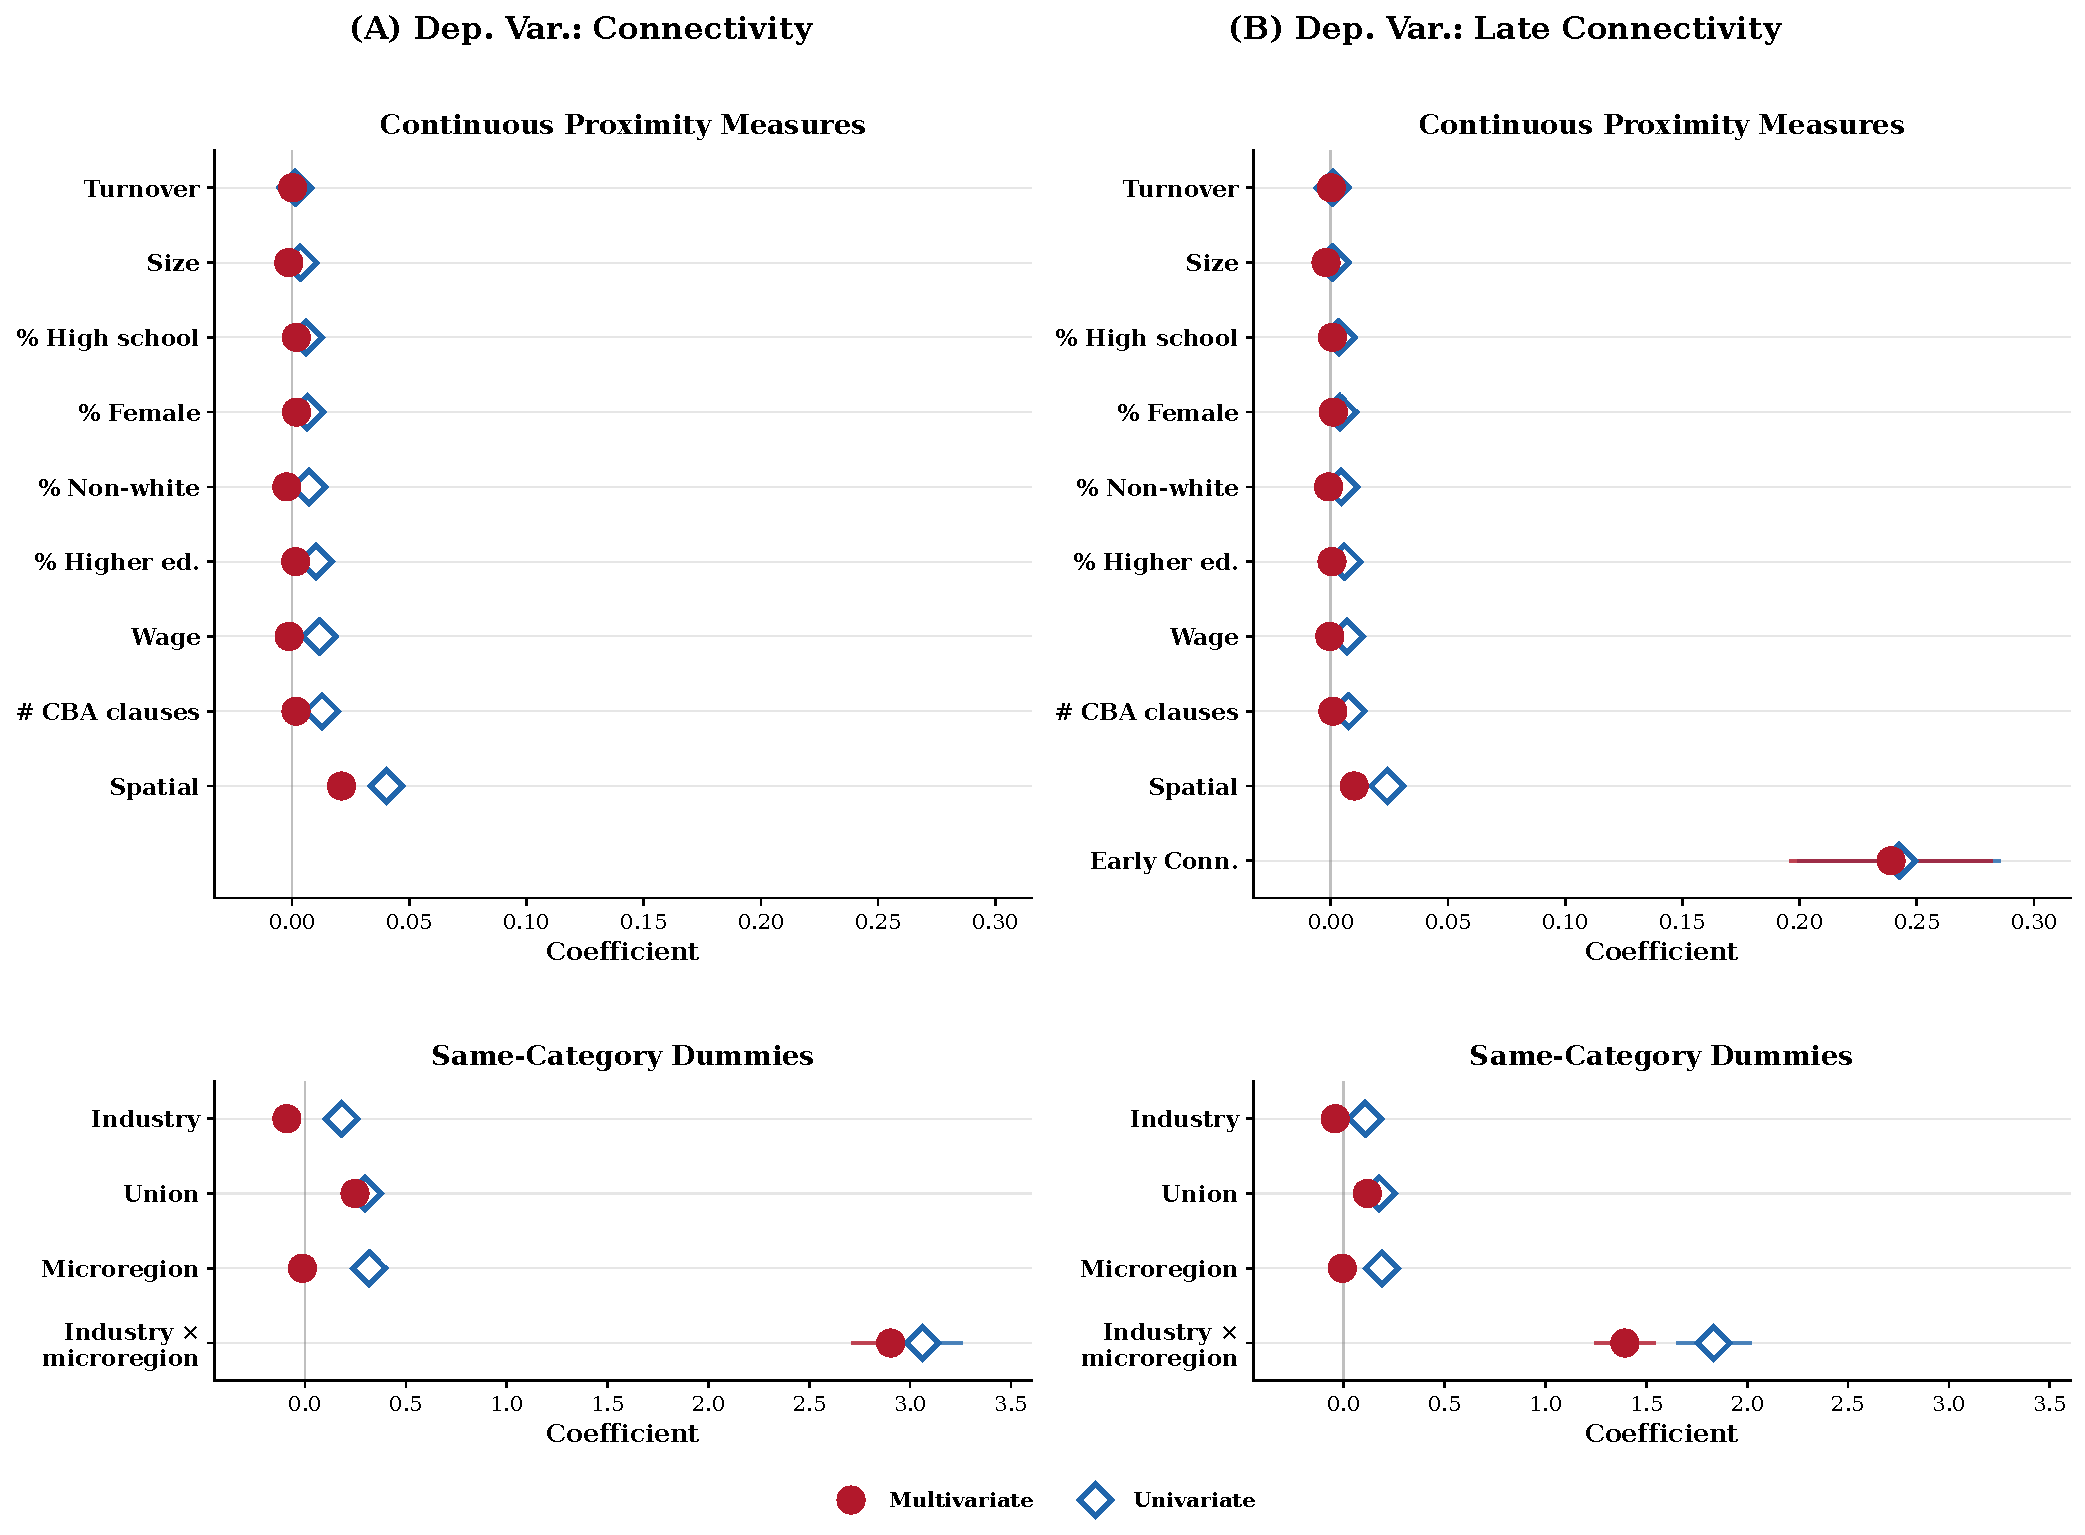
\includegraphics[width=\textwidth]{coefplot_bilateral_combined.pdf}

\begin{tablenotes}
\footnotesize
\item \textit{Notes:} This figure compares predictors of bilateral connectivity across two specifications. Panel~(A) shows regressions where the dependent variable is post-treatment bilateral connectivity (2012--2016). Panel~(B) shows regressions where the dependent variable is late pre-treatment bilateral connectivity (2010--2011); these regressions include ``Early Conn.'' (early pre-treatment connectivity, 2007--2009) as an additional predictor to examine temporal persistence. The top row displays continuous proximity measures; the bottom row displays same-category dummies (binary indicators). Hollow blue diamonds show univariate regressions (each predictor separately); filled red circles show a single multivariate regression including all predictors simultaneously. All regressions include establishment $i$ fixed effects with standard errors two-way clustered by establishment $i$ and establishment $j$. Bilateral connectivity is measured as the person-weighted average flow of workers between establishment pairs. Proximity measures are defined as the negative absolute difference between establishment characteristics (standardized), so higher values indicate greater similarity. Spatial proximity is measured as the negative log of geodesic distance between establishment postal code (CEP) centroids. CBA clauses proximity is the negative absolute difference in the number of collective bargaining agreement clauses. Same-category dummies equal one if both establishments share the indicated category. All establishment characteristics are based on pre-treatment averages. Horizontal lines represent 95\% confidence intervals. $N = 254{,}482{,}256$ establishment pairs.
\end{tablenotes}

\end{threeparttable}
\end{figure}
